% Native editable composition from one verified, unchanged IDE capture.
\begin{figure}[htbp]
\centering
\sbox0{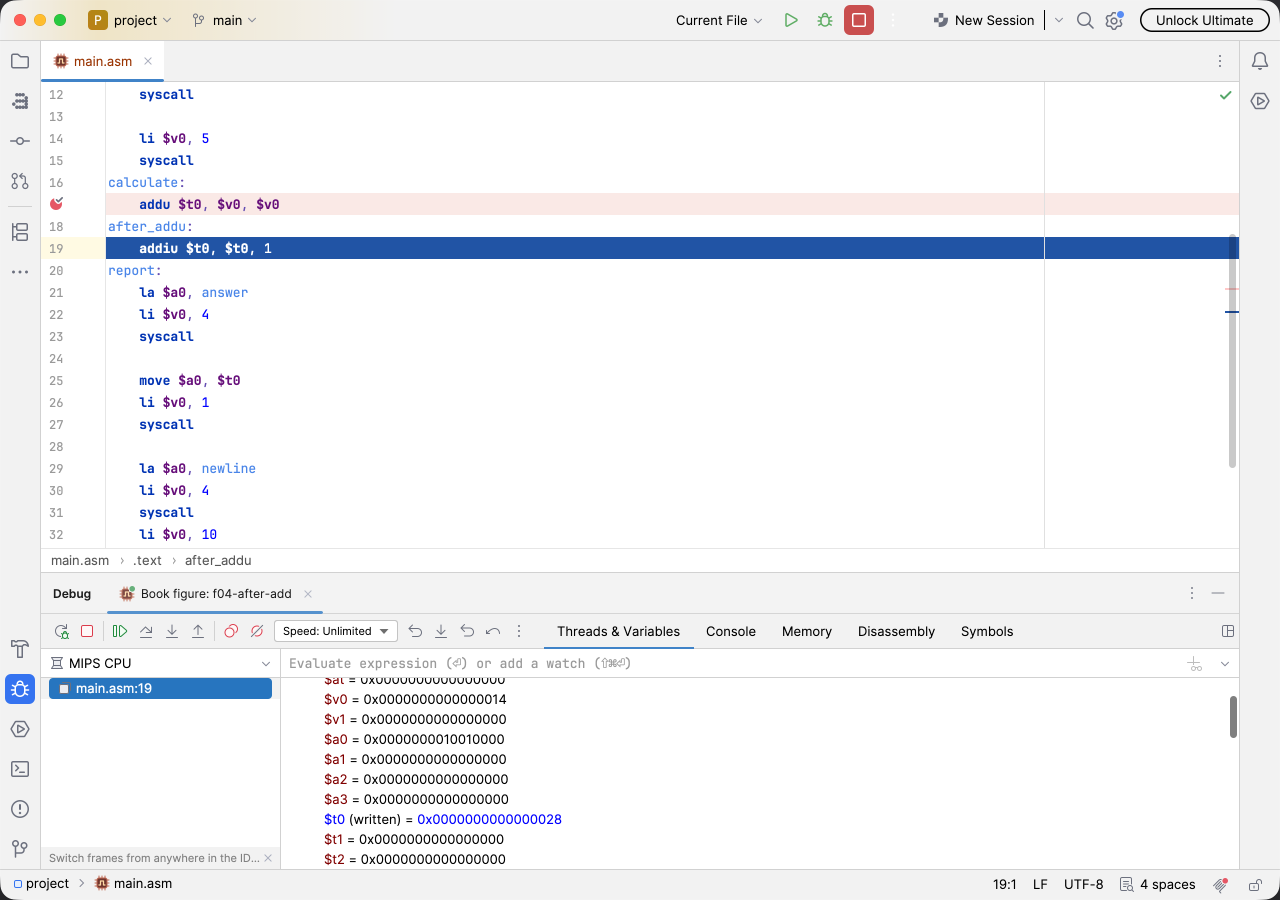
\includegraphics[artifact]{packages/001-console-calculation/captures/f04-after-add/raw.png}}
\edef\MARSconsoleafteraddsourceLeft{\the\dimexpr0.036718750\wd0\relax}
\edef\MARSconsoleafteraddsourceBottom{\the\dimexpr0.707777778\ht0\relax}
\edef\MARSconsoleafteraddsourceRight{\the\dimexpr0.611718750\wd0\relax}
\edef\MARSconsoleafteraddsourceTop{\the\dimexpr0.210000000\ht0\relax}
\edef\MARSconsoleafteraddvalueLeft{\the\dimexpr0.246093750\wd0\relax}
\edef\MARSconsoleafteraddvalueBottom{\the\dimexpr0.075555556\ht0\relax}
\edef\MARSconsoleafteraddvalueRight{\the\dimexpr0.555468750\wd0\relax}
\edef\MARSconsoleafteraddvalueTop{\the\dimexpr0.895555556\ht0\relax}
\begin{tikzpicture}[alt={Two annotated Debug details after the doubling instruction. The next blue source line is addiu t0 t0 one at after_addu. Register t0 is hexadecimal 0000000000000028, decimal 40. The old breakpoint is on the earlier addu line; the current execution line is the later addiu.}]
\node[anchor=north west,inner sep=0,font=\small\bfseries] (source-title) at (6mm,0) {The next instruction adds one};
\node[anchor=north west,inner sep=0] (source) at ([yshift=-1mm]source-title.south west) {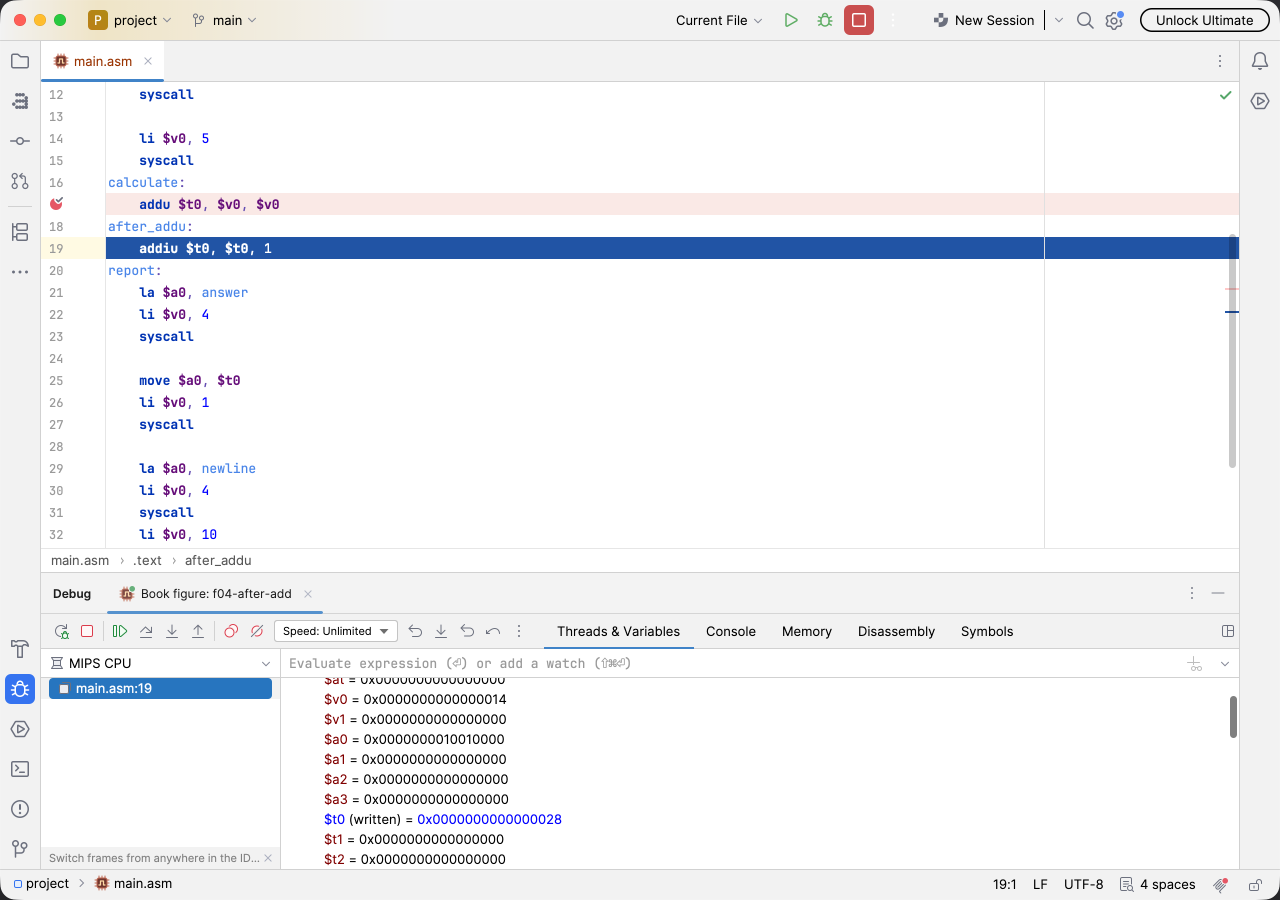
\includegraphics[width=0.7\linewidth,artifact,trim={\MARSconsoleafteraddsourceLeft{} \MARSconsoleafteraddsourceBottom{} \MARSconsoleafteraddsourceRight{} \MARSconsoleafteraddsourceTop{}},clip]{packages/001-console-calculation/captures/f04-after-add/raw.png}};
\begin{scope}[shift={(source.south west)},x={($(source.south east)-(source.south west)$)},y={($(source.north west)-(source.south west)$)}]
\draw[black,line width=0.7pt] (0.135555556,0.054054054) rectangle (0.497777778,0.351351351);
\node[draw=black,fill=white,circle,inner sep=1.5pt,font=\footnotesize] at ($(0.135555556,0.351351351)+(-3mm,0)$) {1};
\end{scope}
\node[anchor=north west,inner sep=0,font=\small\bfseries] (value-title) at ([yshift=-2mm]source.south west) {The intermediate value is decimal 40};
\node[anchor=north west,inner sep=0] (value) at ([yshift=-1mm]value-title.south west) {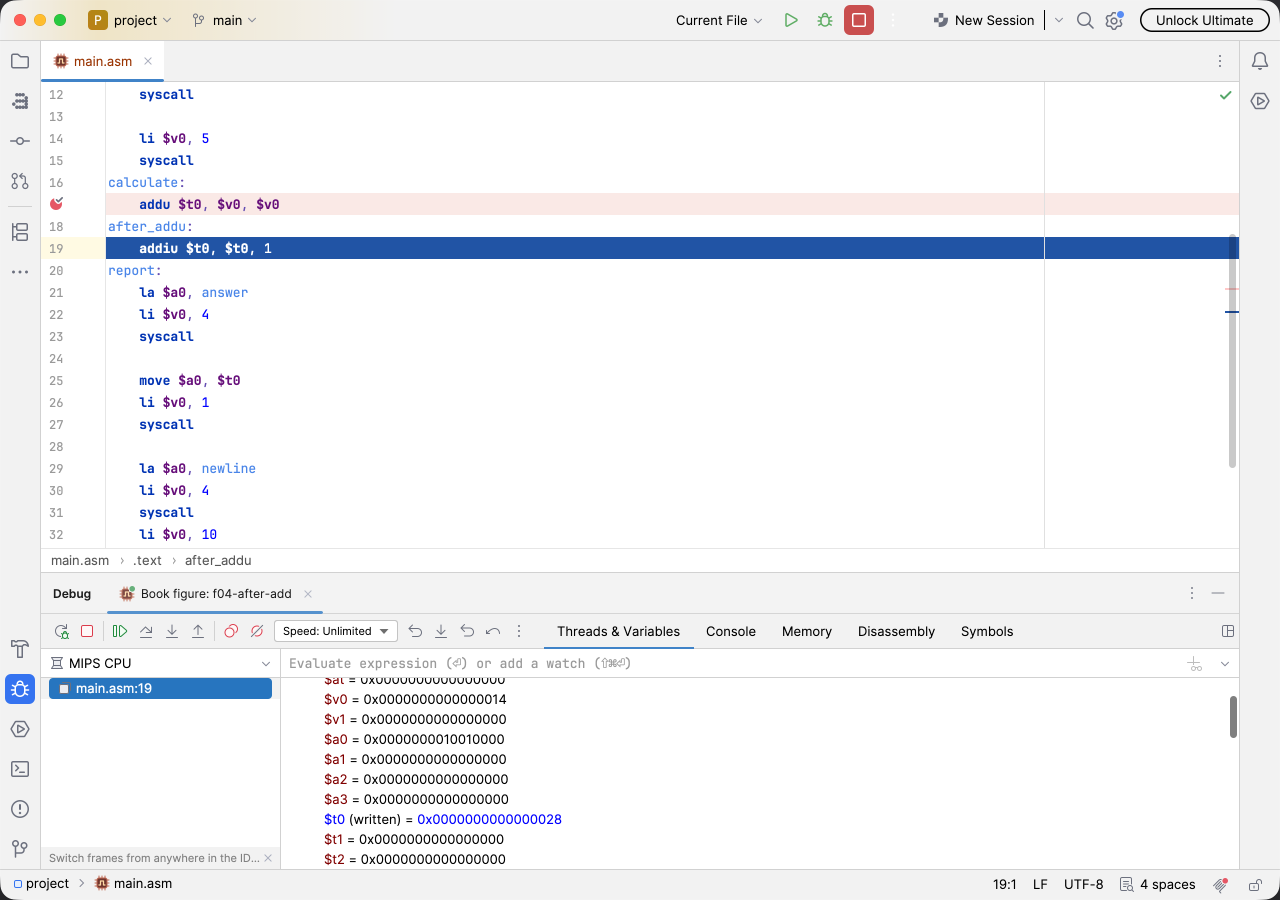
\includegraphics[width=0.53\linewidth,artifact,trim={\MARSconsoleafteraddvalueLeft{} \MARSconsoleafteraddvalueBottom{} \MARSconsoleafteraddvalueRight{} \MARSconsoleafteraddvalueTop{}},clip]{packages/001-console-calculation/captures/f04-after-add/raw.png}};
\begin{scope}[shift={(value.south west)},x={($(value.south east)-(value.south west)$)},y={($(value.north west)-(value.south west)$)}]
\draw[black,line width=0.7pt] (0.023622047,0.115384615) rectangle (0.976377953,0.884615385);
\node[draw=black,fill=white,circle,inner sep=1.5pt,font=\footnotesize] at ($(0.023622047,0.884615385)+(-3mm,0)$) {2};
\end{scope}
\end{tikzpicture}
\par\smallskip
\begin{minipage}{\linewidth}
\small
\begin{enumerate}
\item One Step Over executes the \texttt{addu}. The blue execution line advances to \texttt{addiu \$t0, \$t0, 1}, which has not executed yet. The earlier breakpoint marker remains at the doubling instruction.
\item \texttt{\$t0}=\texttt{0x28}=40. This is the intermediate sum $20+20$; the final addition is still pending.
\end{enumerate}
\end{minipage}
\caption{After one native Debug step over addu. The next instruction will add one.}
\label{capture:001-console-calculation-f04-after-add}
\end{figure}
